\section{Interpretation}
\label{sec:interpretation}

% TODO (group writes the text). Cover (notebooks/04_interpretacao.ipynb):
% - SHAP of the tuned Gradient Boosting: global importance (reports/results/shap_importance.csv,
%   Figure~\ref{fig:shap}) and what the main attributes mean.
% - Variants A/B/C (with administrative network / without / without network and school meals):
%   Table~\ref{tab:variants}, source reports/results/interpretacao_variantes.csv.
% - Residual analysis by network x region (Figure~\ref{fig:resid}), e.g. federal schools
%   over/under-predicted by region.
% - Linear model coefficients and residuals if useful: linreg_coefficients.png, linreg_residuals.png.
% - Limitations: structural features are proxies of socioeconomic status; no causal claim.

\begin{figure}[ht]
  \centering
  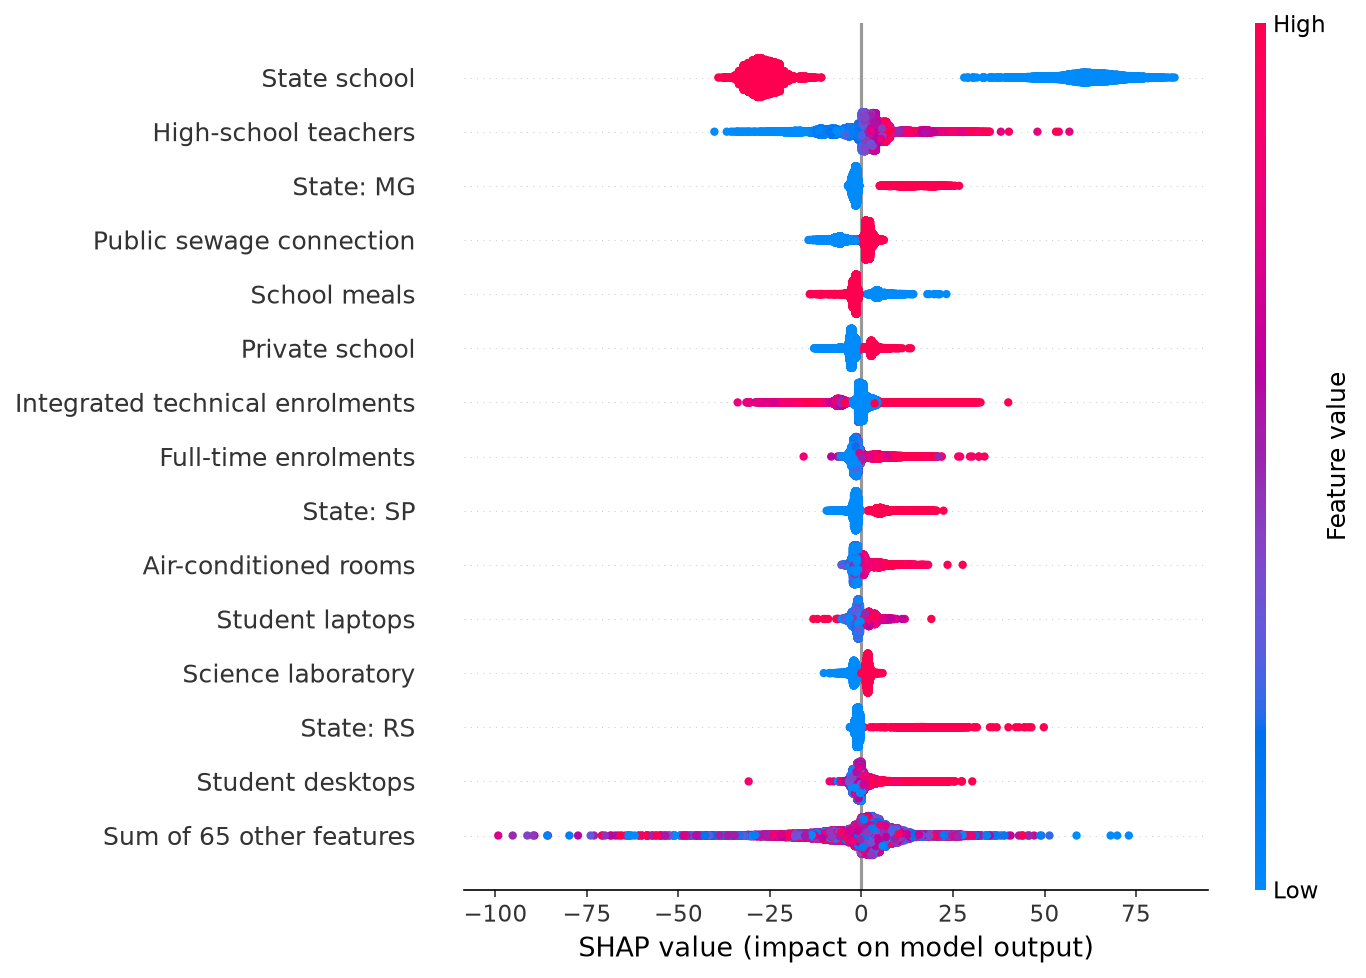
\includegraphics[width=0.8\textwidth]{shap_beeswarm.png}
  \caption{TODO: caption -- SHAP summary (beeswarm) of the tuned Gradient Boosting.}
  \label{fig:shap}
\end{figure}

\begin{table}[ht]
  \centering
  \caption{TODO: caption -- feature-set variants A/B/C, Gradient Boosting vs.\ linear regression.}
  \label{tab:variants}
  \begin{tabular}{llll}
\toprule
Variant & Model & RMSE & $R^2$ \\
\midrule
A & Gradient Boosting & 30.63 $\pm$ 0.90 & 0.76 $\pm$ 0.01 \\
A & Linear & 34.24 $\pm$ 1.15 & 0.70 $\pm$ 0.01 \\
B & Gradient Boosting & 32.46 $\pm$ 1.12 & 0.73 $\pm$ 0.01 \\
B & Linear & 37.32 $\pm$ 1.34 & 0.64 $\pm$ 0.01 \\
C & Gradient Boosting & 37.37 $\pm$ 1.35 & 0.64 $\pm$ 0.01 \\
C & Linear & 43.94 $\pm$ 1.53 & 0.50 $\pm$ 0.02 \\
\bottomrule
\end{tabular}

\end{table}

\begin{figure}[ht]
  \centering
  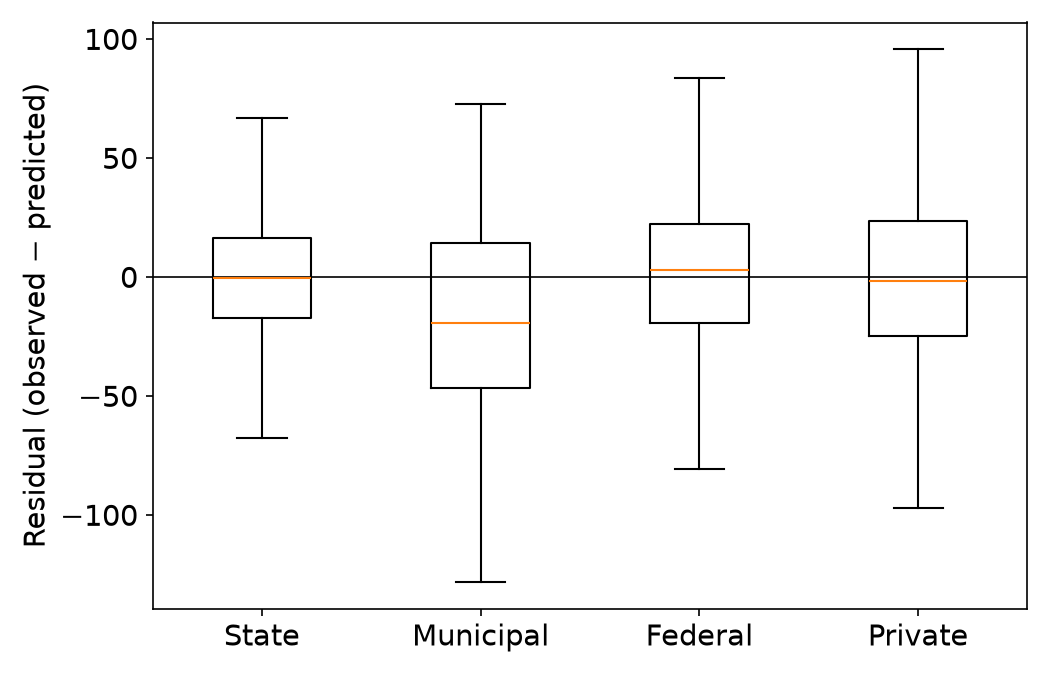
\includegraphics[width=0.8\textwidth]{interpretacao_residuos.png}
  \caption{TODO: caption -- residuals by administrative network and region.}
  \label{fig:resid}
\end{figure}
